\documentclass{article}
% For math environments
\usepackage{amsmath, amsfonts}
% For links
\usepackage[colorlinks=true,
    linkcolor = blue,
    urlcolor  = blue,
    citecolor = blue,
    anchorcolor = blue]{hyperref}
% Put space between paragraphs
\usepackage{parskip}
% For figures
\usepackage{tikz}
% Set the margins to not be ridiculous
\usepackage[margin=0.75in]{geometry}
% For multiple columns
\usepackage{multicol}
% For controlling enum/itemize spacing and indentation
\usepackage{enumitem}
% More math symbols
\usepackage{amssymb}
% To change enumerate labels

% For tikz plots
\usepackage{pgfplots}
% This isn't needed but avoids a compiler warning
\pgfplotsset{compat=1.16}

% Allow multi-line equations to be broken across pages
\allowdisplaybreaks

% Use @ as a letter
\makeatletter

% Scale down all tikz coordinates while maintaining font size
\tikzset{every picture/.style={scale=0.45, every picture/.style={}}}


% Macros
% Monospace code
\def\code#1{\texttt{#1}}

% Greek letters
\def\a{\alpha}
\def\b{\beta}
\def\g{\gamma}
\def\d{\delta}
\def\D{\Delta}

% Commands that make life easier
\newcommand\gath[1]{\begin{gather} #1 \end{gather}}
\newcommand\ali[1]{\begin{align} #1 \end{align}}
\newcommand\parens[1]{\left( #1 \right)}
\newcommand\squares[1]{\left[ #1 \right]}
\newcommand\braces[1]{\left\{ #1 \right\}}
\newcommand\angles[1]{\left\langle #1 \right\rangle}
\newcommand\deriv[2]{\frac{d #1}{d #2}}
\newcommand\abs[1]{\left| #1 \right|}
\newcommand\floor[1]{\left\lfloor #1 \right\rfloor}
\DeclareMathOperator{\lcm}{lcm}
\def\non{\nonumber \\}

% Multiline equation space
\def\mlesp{\hspace{1.2cm}}

% For grid diagrams
\newcommand\gridbox[3]{\draw (#1,#2) rectangle (#1+1,#2+1) node[pos=.5] {#3};}
\newcommand\gridboxh[3]{\draw[fill=red!20] (#1,#2) rectangle (#1+1,#2+1) node[pos=.5] {#3};}
\newcommand\gridboxb[3]{\draw[fill=black] (#1,#2) rectangle (#1+1,#2+1) node[pos=.5] {#3};}
\newcommand\gridsym[3]{\node at (#1+0.5,#2+0.5) {$#3$};}
\newcommand\gridblank[2]{\filldraw[draw=gray, color=gray] (#1,#2) rectangle (#1+1,#2+1);}
\newcommand\gridcirc[2]{\draw (#1 + 0.5,#2 + 0.5) circle (0.25);}
\newcommand\cwlab[3]{
  \def\dd{0.15}
  \draw (#1 + \dd - 0.03, #2 + 1 - \dd) node {\scriptsize #3};
}

\def\bbw{3.5}
\def\bbh{2}
\newcommand\bigbox[3]{\draw (#1*\bbw,#2*\bbh) rectangle (#1*\bbw+\bbw,#2*\bbh+\bbh) node[pos=.5] {#3};}
\newcommand\bbtextr[3]{\node[right] at (#1*\bbw,#2*\bbh+0.5*\bbh) {#3};}
\newcommand\bbtextb[3]{\node[align=center] at (#1*\bbw+0.5*\bbw,#2*\bbh+0.5*\bbh) {#3};}

% Box puzzle stock answer
\newcommand\boxans[1]{
  Logic was used to deduce the solution:

  #1

  This was verified using Python as well as shown to be unique with a brute force approach.
}

% Multiple numbers
\newcommand\mn[1]{$#1$'s}

% Commands for problems
\newcommand\problem[4]{
  \section*{#1}

  Question: #3
  
  Answer: #2
  
  Explanation: #4
}
\newcommand\aproblem[4]{\problem{Dec #1}{#2}{#3}{#4}}
\newcommand\cproblem[4]{\problem{Problem #1}{#2}{#3}{#4}}

\def\advent@xxiv@i{
  Eve writes down five different positive integers.
  The sum of her integers is $16$. What is the product of her integers?
}

\def\advent@xxiv@ii{
  $14$ is the smallest even number that cannot be obtained by rolling two $6$-sided dice and finding the product of the numbers rolled.

  What is the smallest even number that cannot be obtained by rolling one hundred $100$-sided dice and finding the product of the numbers rolled?
}

\def\advent@xxiv@iii{
  There are $5$ ways to write $5$ as the sum of positive odd numbers:
  \begin{itemize}
    \item $1 + 1 + 1 + 1 + 1$
    \item $1 + 1 + 3$
    \item $3 + 1 + 1$
    \item $1 + 3 + 1$
    \item $5$
  \end{itemize}

  How many ways are there to write $14$ as the sum of positive odd numbers?
}

\def\advent@xxiv@iv{
  The geometric mean of a set of $n$ numbers is computed by mulitplying all the numbers together, then taking the $n$th root.
  The factors of $9$ are $1$, $3$, and $9$.
  The geometric mean of these factors is
  \gath{
    \sqrt[3]{1 \times 3 \times 9} = \sqrt[3]{27} = 3
  }
  What is the smallest number where the geometric mean of its factors is $13$?
}

\def\advent@xxiv@v{
  The sum of $11$ consecutive integers is $2024$.
  What is the smallest of the $11$ integers?
}

\def\advent@xxiv@vi{Put the digits 1 to 9 (using each digit exactly once) in the boxes so that the sums are correct. The sums should be read left to right and top to bottom ignoring the usual order of operations. For example, 4+3×2 is 14, not 10. Today's number is the product of the numbers in the red boxes.
  The number $n$ has $55$ digits.
  All of its digits are $9$.
  What is the sum of the digits of $n^3$?
}

\def\advent@xxiv@vii{
  What is the obtuse angle in degrees between the minute and hour hands of a clock at 08:22?
}

\def\advent@xxiv@viii{
  It is possible to arrange $4$ points on a plane and draw non-intersecting lines between them to form $3$ non-overlapping triangles:

  \begin{center}
    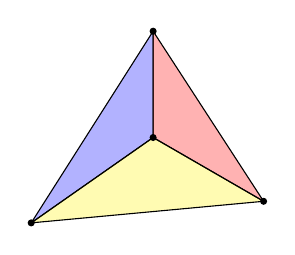
\begin{tikzpicture}
      \def\ds{3}
      \def\pa{(0: 0)}
      \def\pb{(90: \ds)}
      \def\pc{(215: 1.4*\ds)}
      \def\pd{(-30: 1.2*\ds)}

      \def\bcr{3}
      \def\scr{0.55*\bcr}
      \def\sca{34}
      \def\mcr{0.7*\bcr}
      \def\mca{142}
      \def\pr{0.1}

      % Triangles
      \draw[fill=blue,fill opacity=0.3] \pa -- \pb -- \pc -- cycle;
      \draw[fill=red,fill opacity=0.3] \pa -- \pb -- \pd -- cycle;
      \draw[fill=yellow,fill opacity=0.3] \pa -- \pd -- \pc -- cycle;

      % Points
      \fill \pa circle (\pr);
      \fill \pb circle (\pr);
      \fill \pc circle (\pr);
      \fill \pd circle (\pr);
    \end{tikzpicture}
  \end{center}

  It is not possible to make more than $3$ triangles with $4$ points.

  What is the maximum number of non-overlapping triangles that can be made by arranging $290$ points on a plane and drawing non-intersecting lines between them?
}

\def\advent@xxiv@ix{
  Put the digits $1$ to $9$ (using each digit exactly once) in the boxes so that the sums are correct.
  The sums should be read left to right and top to bottom ignoring the usual order of operations.
  For example, $4 + 3 \times 2$ is $14$, not $10$.
  Today's number is the product of the numbers in the red boxes.

  \grid@advent@xxiv@ix{}{}{}{}{}{}{}{}{}
}

\def\advent@xxiv@x{
  A number is a palindrome if it's the same when its digits are written in reverse order.

  What is the sum of all the numbers between $10$ and $100$ that are palindromes?
}

\def\advent@xxiv@xi{
  There are $6$ sets of integers between $1$ and $5$ (inclusive) that contain an odd number of numbers whose median value is $3$:

  \begin{itemize}
    \item $\braces{3}$
    \item $\braces{1,3,4}$
    \item $\braces{2,3,4}$
    \item $\braces{1,3,5}$
    \item $\braces{2,3,5}$
    \item $\braces{1,2,3,4,5}$
  \end{itemize}

  How many sets of integers between $1$ and $11$ (inclusive) are there that contain an odd number of numbers whose median value is $5$?
}

\def\advent@xxiv@xii{
  Holly picks a three-digit number.
  She then makes a two-digit number by removing one of the digits.
  The sum of her two numbers is $309$.
  What was Holly's original three-digit number?
}

\def\advent@xxiv@xiii{
  Today's number is given in this crossnumber.
  No number in the completed grid starts with $0$.

  \begin{multicols}{2}
    \crossnumstd{}{}{}{}{}{}{}{}{}

    \vfill\null
    \columnbreak

    \begin{center}
      \textbf{Across}

      \begin{tabular}{clc}
        \textbf{1} & Today's number.  & (\textbf{3}) \\
        \textbf{4} & Two times 5A.    & (\textbf{3}) \\
        \textbf{5} & A multiple of 1. & (\textbf{3})
      \end{tabular}

      \textbf{Down}

      \begin{tabular}{clc}
        \textbf{1} & Sum of digits is 15. & (\textbf{3}) \\
        \textbf{2} & Sum of digits is 19. & (\textbf{3}) \\
        \textbf{3} & Three times 5A.      & (\textbf{3})
      \end{tabular}
    \end{center}
  \end{multicols}
}

\def\advent@xxiv@xiv{
  $15^3$ is $3375$.
  The last $3$ digits of $15^3$ are $375$.

  What are the last $3$ digits of $15^{1234567890}$?
}

\def\advent@xxiv@xv{
  The number $2268$ is equal to the product of a square number (whose last digit is not $0$) and the same square number with its digits reversed: $36 \times 63$.

  What is the smallest three-digit number that is equal to the product of a square number (whose last digit is not $0$) and the same square number with its digits reversed?
}

\def\advent@xxiv@xvi{
  Put the digits $1$ to $9$ (using each digit exactly once) in the boxes so that the sums are correct.
  The sums should be read left to right and top to bottom ignoring the usual order of operations.
  For example, $4 + 3 \times 2$ is $14$, not $10$.
  Today's number is the product of the numbers in the red boxes.

  \grid@advent@xxiv@xvi{}{}{}{}{}{}{}{}{}
}

\def\advent@xxiv@xvii{
  The number $40$ has $8$ factors: $1$, $2$, $4$, $5$, $8$, $10$, $20$, and $40$.

  How many factors does the number $2^{26} \times 5 \times 7^5 \times 11^2$ have?
}

\def\advent@xxiv@xviii{
  TODO
}

\def\card@xxiv@i{
  What is the largest number you can make by using the digits $1$ to $4$ to make two $2$-digit numbers, then mutiplying the two numbers together?
}

\def\card@xxiv@ii{
  What is the largest number you can make by using the digits $0$ to $9$ to make a $2$-digit number and an $8$-digit number, then mutiplying the two numbers together?
}

\def\card@xxiv@iii{
  The expansion of $(2x+3)^2$ is $4x^2 + 12x + 9$.
  The sum of the coefficients of $4x^2 + 12x + 9$ is $25$.
  What is the sum of the coefficients of the expansion of $(30x + 5)^2$?
}

\def\card@xxiv@iv{
  What is the sum of the coefficients of the expansion of $(2x+1)^{11}$?
}

\def\card@xxiv@v{
  What is the geometric mean of all the factors of $41306329$?
}

\def\card@xxiv@vi{
  What is the largest number for which the geometric mean of all its factors is $92$?
}

\def\card@xxiv@vii{
  What is the sum of all the factors of $7^4$?
}

\def\card@xxiv@viii{
  How many numbers between $1$ and $28988500000$ have an odd number of factors?
}

\def\card@xxiv@ix{
  Eve found the total of the $365$ consecutive integers starting at $500$ and the total of the next $365$ consecutive integers, then subtracted the smaller total from the larger total.
  What was her result?
}

\def\card@xxiv@x{
  Eve found the total of the $n$ consecutive integers starting at a number and the total of the next $n$ consecutive integers, then subtracted the smaller total from the larger total.
  Her result was $22344529$.
  What is the largest possible value of $n$ that she could have used?
}

\input{boxes}

% Used for right angle boxes
\usepackage{tkz-euclide}

\begin{document}

\title{MS Scroggs Advent Calendar 2022 Answers}
\author{Dan Whitman}
\date{}

\maketitle

% TODO: Once the event is over, add answers link.
%Answers: \href{https://www.mscroggs.co.uk/puzzles/advent2021}{https://www.mscroggs.co.uk/puzzles/advent2021}
Synchronized calendar: \href{http://mscroggs.co.uk/adventcode/JYcziCbI}{http://mscroggs.co.uk/adventcode/JYcziCbI}

\aproblem{1}{162}{\advent@xxii@i}{
  Since $p_1 = (9,0)$ is a vertex and the $y$-axis is a line of symmetry, it must be that a second vertex is $p_2 = (-9, 0)$.
  Since there must be four vertices, and both $p_1$ and $p_2$ are on the $x$-axis, it must be that the other two vertices are on the $y$-axis.
  This is because any vertex not on either axis would result in four vertices not on either axis due to the axes being lines of symmetry, and a rectangle cannot have six vertices!
  It then must be that the two $y$-axis vertices are at $p_3 = (0, 9)$ and $p_4 = (0, -9)$, since any other points that possess the required symmetry would result in a parallelogram without right angles.

  Therefore, our rectangle is also square that clearly has sides of $s = \sqrt{9^2 + 9^2} = 9\sqrt{2}$.
  The area is then of course $A = s^2 = 81 \cdot 2 = 162$.
}

\aproblem{2}{840}{\advent@xxii@ii}{
  Clearly $1$, $2$, $3$, $5$, and $7$ are prime whereas $4 = 2^2$, $6 = 2 \cdot 3$, and $8 = 2^3$.
  Therefore we have that
  \gath{
    \lcm(1, 2, 3, 4, 5, 6, 7, 8) = 2^3 \cdot 3 \cdot 5 \cdot 7 = 840 \,.
  }
}

\aproblem{3}{369}{\advent@xxii@iii}{
  Suppose that for the $n$th row we choose the element in the $p_n$th column (where $1 \leq n, p_n \leq 9$).
  Since we must only choose exactly one number in each column, clearly for any permutation we have that $\braces{p_n \mid 1 \leq n \leq 9} = \braces{1, 2, \ldots, 9}$, and hence
  \gath{
    \sum_{n=1}^9 p_n = 1 + 2 + \ldots + 9 = \sum_{i=1}^9 i = \frac{9 \cdot 10}{2} = 45 \,.
  }
  Now, if $x_n$ is the selected value of the $n$th row, then this value is reasoned to be
  \gath{
    x_n = 9(n-1) + p_n \,.
  }
  Hence, the sum of all the selected values is always
  \gath{
    \sum_{n=1}^9 x_n = \sum_{n=1}^9 \squares{9(n-1) + p_n} = 9 \sum_{n=1}^9 n - 9 \sum_{n=1}^9 1 + \sum_{n=1}^9 p_n
    = 9 \cdot 45 - 9 \cdot 9 + 45 = 369
  }
  regardless of the selection permutation.
  This result was verified by a brute force Python program.
}

\aproblem{4}{625}{\advent@xxii@iv}{
  First, clearly the last three digits of any number $n \geq 100$ is just $n \mod 1000$.
  We claim, for all $n \geq 3$, that
  \gath{
    5^n \mod 1000 = \begin{cases}
      625 & \text{$n$ is even}    \\
      125 & \text{$n$ is odd} \,,
    \end{cases}
  }
  which we show by induction on $n$.
  First, for $n = 3$, we obviously have $5^3 = 125 \equiv 125 \pmod{1000}$ so that the hypothesis is true here since $n = 3$ is odd.
  Now suppose that the hypothesis is true for $n$.
  If $n$ is even then $5^n \equiv 625 \pmod{1000}$ so that
  \gath{
    5^{n+1} = 5 \cdot 5^n \equiv 5 \cdot 625 \pmod{1000} \equiv 3125 \pmod{1000} \equiv 125 \pmod{1000},
  }
  which proves the hypothesis for $n+1$ since $n+1$ is odd.
  If, on the other hand, $n$ is odd, then $5^n \equiv 125 \pmod{1000}$ by the induction hypothesis so that
  \gath{
    5^{n+1} = 5 \cdot 5^n \equiv 5 \cdot 125 \pmod{1000} \equiv 625 \pmod{1000},
  }
  which again proves the hypothesis for $n+1$ since here $n+1$ is even.

  Now, since clearly $n = 2022000000$ is even, it follows that the last three digits of $5^n$ are $625$ by what was just proven.
}

\aproblem{5}{315}{\advent@xxii@v}{
  \boxans{\gridsol@advent@xxii@v}
}

\aproblem{6}{128}{\advent@xxii@vi}{
  First, consider a general sum digit $1 \leq s \leq 9$, and let $N_m(s)$ denote the number of $m$-digit numbers such that the digits are all non-zero digits and add to $s$.
  Clearly $N_1(s) = 1$, namely the single digit $s$ itself.
  Next, consider $m$-digit numbers for $m > 1$.
  If the first digit is $1$, then there are $N_{m-1}(s-1)$ combinations of remaining digits so that to overall digital sum is $s$.
  Likewise, if the first digit is $2$, then there are $N_{m-1}(s-2)$ combinations of remaining digits.

  More generally, if the first digit is $1 \leq i \leq s - (m-1)$, then there are $N_{m-1}(s - i)$ combinations of remaining digits such that the overall digital sum is $s$.
  Note that $i \leq s - (m-1)$ since the minimal sum of the remaining digits is $m-1$, namely when they are all \mn{1}.
  Therefore, considering all the first digits, we have the recursive equation
  \gath{
    N_m(s) = \sum_{i=1}^{s - (m-1)} N_{m-1}(s - i) = \sum_{j=m-1}^{s-1} N_{m-1}(j), \label{eqn:06:rec}
  }
  where we have changed indices using $j = s - i$.
  Also note that it must be that $m \leq s$ since there are no terms otherwise, and $m = s$ corresponds to an $s$-digit number with a digital sum $s$ so that all digits must be \mn{1}, and hence $N_s(s) = 1$.

  For a given $s$, it follows that the total number of qualifying integers (with any number of digits) with that digital sum is then
  \gath{
    N_s = \sum_{m=1}^s N_m(s). \label{eqn:06:main}
  }
  Now, we have
  \gath{
    N_2(s) = \sum_{j=1}^{s-1} N_1(j) = \sum_{j=1}^{s-1} 1 = (s - 1) - 1 + 1 = s - 1
  }
  and
  \ali{
    N_3(s) &= \sum_{j=2}^{s-1} N_2(j) = \sum_{j=2}^{s-1} (s - 1) = \sum_{j=2}^{s-1} s - \sum_{j=2}^{s-1} 1 = \squares{\frac{s(s-1)}{2} - 1} - (s - 2) \non
    &= \frac{s(s-1)}{2} - s + 1 = \frac{s(s-1) - 2s + 2}{2} = \frac{s^2 - 3s + 2}{2} = \frac{(s-1)(s-2)}{2}.
  }
  This could be continued to $N_4(s)$, $N_5(s)$, etc., but this would quickly become very tedious.
  In our case we are looking for $N_8$, for which we would need to determine $N_m(s)$ up through $N_8(s)$.
  Rather than endure this tedium, we simply implement the recursive function \eqref{eqn:06:rec} with the base case of $N_1(s) = 1$ in Python and use \eqref{eqn:06:main} to calculate $N_8 = 128$.

  This result was also verified with a brute force search in the Python program.
}

\aproblem{7}{476}{\advent@xxii@vii}{
  It seems fairly clear that the largest triangle that can fit within a hexagon is that whose three vertices lie on every other vertex of the hexagon as shown below:
  \def\hexr{3}
  \begin{center}
    \begin{tikzpicture}
      \draw (-30:\hexr) -- (30:\hexr) -- (90:\hexr) -- (150:\hexr) -- (210:\hexr) -- (270:\hexr) -- cycle;
      \draw[fill=red] (-30:\hexr) -- (90:\hexr) -- (210:\hexr) -- cycle;
    \end{tikzpicture}
  \end{center}
  Let $s$ denote the side length of the hexagon, and let $t$ denote the side of the inner red triangle, which is clearly equilateral.
  The three smaller white triangles inside the hexagon but outside the red triangle are isosceles and have two side of length $s$ and a base of length $t$.
  Moreover, the apex angles of these triangles is $120^\circ$, from which it follows that
  \gath{
    t = \sqrt{3} s
  }
  so that the area of the large red triangle is
  \gath{
    A_t = \frac{\sqrt{3}}{4} t^2 = \frac{\sqrt{3}}{4} \parens{\sqrt{3} s}^2 = \frac{3\sqrt{3}}{4} s^2.
  }
  Meanwhile, the area of the hexagon is
  \gath{
    A_h = \frac{3\sqrt{3}}{2} s^2.
  }
  Therefore, we have
  \gath{
    A_t = \frac{1}{2} A_h = \frac{1}{2} \cdot 952 = 476.
  }
}

\aproblem{8}{840}{\advent@xxii@viii}{
  Suppose that the five real roots are $a$, $b$, $c$, $d$, and $e$ so that the quintic equation is then of course
  \gath{
    (x - a)(x - b)(x - c)(x - d)(x - e) = 0.
  }
  If we were to expand this, clearly the last term is the only term to be a constant without a factor of $x$.
  This expansion would thus have the form
  \gath{
    f(x) + abcde = 0
  }
  such that $f(x)$ is some quintic in which every term has a factor of $x$.
  Therefore, $-f(x) = abcde$, which is exactly the form of the original given equation.
  Hence, the right side is the product of all the roots, which is the answer we seek!

  While not necessary to get the sought answer, we can also use this and a bit of trial and error to quickly and easily find what the roots actually are.
  Our root product $840$ has 32 factors, not including $840$ itself.
  So the roots can be determined by just plugging all the factors into the original quintic and see which result in the equation holding, being careful to also try the negatives of the factors as well.
  This tedious process was implemented in Python to arrive at the five distinct roots $\braces{-4, -3, 2, 5, 7}$.
  It was then verified using Wolfram Alpha that fully expanding the quintic $(x + 4)(x + 3)(x - 2)(x - 5)(x - 7)$ indeed results in the original quintic expression.
}

\aproblem{9}{532}{\advent@xxii@ix}{
  \boxans{\gridsol@advent@xxii@ix}
}

\aproblem{10}{800}{\advent@xxii@x}{
  \def\xmin{\frac{a}{2}}
  Let $f(x) = x^2 - ax$ and $b = -160,000$.
  Clearly the tangent line $y = b$ is perfectly horizontal so that this touches the parabola $f(x)$ when its slope is zero.
  Thus, we have that this occurs at
  \gath{
    f'(x) = 2x - a = 0 \non
    x = \xmin.
  }
  Now, since the parabola must touch the line at this point, it must be that
  \gath{
    f\parens{\xmin} = \parens{\xmin}^2 - a \parens{\xmin} = b \non
    \frac{a^2}{4} - \frac{a^2}{2} = b \non
    \frac{s^2 - 2a^2}{4} = b \non
    -\frac{a^2}{4} = b \non
    a = \sqrt{-4b} = 800.
  }
  This result was verified by plotting $f(x)$ and the line $y = b$ using Python.
}

\aproblem{11}{987}{\advent@xxii@xi}{
  Let $N_1(m)$ denote the number of qualifying $m$-digit numbers that start with a $1$, and let $N_2(m)$ be the number of qualifying $m$-digit numbers that start with a $2$.
  Similarly, let $N(m)$ denote the total number of qualifying $m$-digit numbers.
  Now, if a $m$-digit number starts with a $1$, then the next digit may either be a $1$ \emph{or} a $2$.
  Thus, it follows that
  \gath{
    N_1(m) = \begin{cases}
      1                   & m = 1  \\
      N_1(m-1) + N_2(m-1) & m > 1.
    \end{cases}
    \label{eqn:11:N1rec}
  }
  On the other hand, if an $m$-digit number starts with a $2$, then the next digit \emph{must} be a $1$ so as not to have two \mn{2} in a row.
  Therefore,
  \gath{
    N_2(m) = \begin{cases}
      1        & m = 1 \\
      N_1(m-1) & m > 1 \\
    \end{cases}
    \label{eqn:11:N2rec}
  }
  and also clearly in general
  \gath{
    N(m) = N_1(m) + N_2(m).
  }
  Combining \eqref{eqn:11:N1rec} and \eqref{eqn:11:N2rec} gives
  \gath{
    N_1(m) = \begin{cases}
      1                                         & m = 1 \\
      N_1(1) + N_2(1) = 2                       & m = 2 \\
      N_1(m-1) + N_2(m-1) = N_1(m-1) + N_1(m-2) & m > 2
    \end{cases}
  }
  Lastly, we generally have
  \gath{
    N(m) = N_1(m) + N_2(m) = N_1(m) + N_1(m-1) = N_1(m+1).
  }
  Hence,
  \gath{
    N(m) = \begin{cases}
      N_1(1) = 1                                     & m = 0  \\
      N_1(2) = 2                                     & m = 1  \\
      N_1(m+1) = N_1(m) + N_1(m-1) = N(m-1) + N(m-2) & m > 1.
    \end{cases}
    \label{eqn:11:Nrec}
  }

  Now, the recursive function $\eqref{eqn:11:Nrec}$ is just a shifted Fibonacci sequence.
  As such, these do have a closed-form solution, but it is a bit nasty and involves powers of the golden ratio and its conjugate.
  Because of this, we simply implement the recursive function in Python and evaluate our answer $N(14) = 987$.

  This result was verified using a brute force Python program.
}

\aproblem{12}{143}{\advent@xxii@xii}{
  \newcommand\maxsub[1]{{#1}_\mathrm{max}}
  For the general $2$ by $2$ matrix
  \gath{
    M = \begin{pmatrix}
      a & b \\
      c & d
    \end{pmatrix}
  }
  the determinant is of course $\abs{M} = ad - bc$.
  So, if we want to maximize this determinant, we should maximize the $ad$ term and minimize the $bc$ term.
  Thus, if $A$ is a finite set of positive integers where $x$ is the lowest number and $y$ is the greatest number and the matrix entries may be chosen from $A$, then clearly the maximum determinant is that of the matrix
  \gath{
    \maxsub{M} = \begin{pmatrix}
      y & x \\
      x & y
    \end{pmatrix}
  }
  so that the maximum determinant is $\abs{\maxsub{M}} = y^2 - x^2$.

  Thus, for the set of entries $\braces{1, 2, 3, ..., 12}$, clearly the least and greatest numbers are $x = 1$ and $y = 12$, respectively.
  It then follows that the maximum determinant we seek is $\abs{\maxsub{M}} = 12^2 - 1^2 = 143$.
}

\aproblem{13}{564}{\advent@xxii@xiii}{
  Logic was used to deduce the solution:
  \grid@advent@xxii@xiii{1}{2}{5}{2}{5}{6}{1}{0}{4}
  In particular, the first column is the square number, the second column is twice the first row, and the third column is today's number.
  The solution was verified with Python.
}

\aproblem{14}{614}{\advent@xxii@xiv}{
  Clearly the fact that each pentagon has a perimeter of $5$ means that each side has a length of $1$.
  Supposing we have at least $3$ pentagons in a line as above, it is easy to reason that the two pentagons on either end contribute $4$ to the perimeter while those in the middle each contribute $3$.
  For $n$ total pentagons, clearly there are always $2$ end pentagons and $n-2$ in the middle.
  So, if we let $P(n)$ denote the perimeter of $n$ pentagons, then we have
  \gath{
    P(n) = 2 \cdot 4 + 3 (n-2) = 8 + 3n - 6 = 3n + 2.
  }
  Interestingly, this formula still works for only one or two pentagons since clearly $P(1) = 5$ and $P(2) = 8$.
  Our answer is of course $P(204) = 614$.
}

\aproblem{15}{243}{\advent@xxii@xv}{
  Suppose we have two odd numbers $a$ and $b$ such that $a < b$.
  Since they are both odd, we have $a = 2n+1$ and $b = 2m+1$ for some integers $n$ and $m$, which of course implies that
  \ali{
    n &= \frac{a-1}{2} & m &= \frac{b-1}{2}.
  }
  Now, clearly the even numbers between $a$ and $b$ range from $2n+2 = 2(n+1)$ to $2m$ inclusive so that there are
  \gath{
    N(a, b) = m - (n+1) + 1 = m - n = \frac{b-1}{2} - \frac{a-1}{2} = \frac{b-a}{2}
  }
  of these even numbers.
  Based on what we are asked to find, we have $b = 729$, and we must find the odd number $a$ such that
  \gath{
    a = N(a, b) = \frac{b-a}{2} \non
    2a = b - a \non
    3a = b \non
    a = \frac{b}{3}
  }
  so that our answer is $a = b/3 = 729/3 = 243$.
}

\aproblem{16}{324}{\advent@xxii@xvi}{
  In the 2021, Dec~11 problem, it deduced that the number of numbers in the $n$th row is $N(n) = 2n-1$, where the first row is $n = 1$.
  It was also shown that the first (i.e. leftmost) number of the $n$th row is
  \gath{
    a_n = n(n - 2) + 2.
  }
  Clearly then the last (i.e. rightmost) number in the $n$th row is then
  \gath{
    b_n = a_{n+1} - 1 = \squares{(n+1)(n-1) + 2} - 1 = (n+1)(n-1) + 1.
  }
  It is then easy to calculate the following tables:
  \begin{multicols}{4}
    \begin{center}
      \begin{tabular}{c|cc}
        $n$ & $a_n$ & $b_n$ \\
        \hline
        1   & 1     & 1     \\
        2   & 2     & 4     \\
        3   & 5     & 9     \\
        4   & 10    & 16    \\
        5   & 17    & 25    \\
      \end{tabular}
    \end{center}
    \columnbreak

    \begin{center}
      \begin{tabular}{c|cc}
        $n$ & $a_n$ & $b_n$ \\
        \hline
        6   & 26    & 36    \\
        7   & 37    & 49    \\
        8   & 50    & 64    \\
        9   & 65    & 81    \\
        10  & 82    & 100   \\
      \end{tabular}
    \end{center}
    \columnbreak

    \begin{center}
      \begin{tabular}{c|cc}
        $n$ & $a_n$ & $b_n$ \\
        \hline
        11  & 101   & 121   \\
        12  & 122   & 144   \\
        13  & 145   & 169   \\
        14  & 170   & 196   \\
        15  & 197   & 225   \\
      \end{tabular}
    \end{center}
    \columnbreak

    \begin{center}
      \begin{tabular}{c|cc}
        $n$ & $a_n$ & $b_n$ \\
        \hline
        16  & 226   & 256   \\
        17  & 257   & 289   \\
        18  & 290   & 324   \\
        19  & 325   & 361   \\
        20  & 362   & 400   \\
      \end{tabular}
    \end{center}
  \end{multicols}

  From these it is clear that $300$ is in row $18$, the rightmost element of which is $324$.
}

\aproblem{17}{144}{\advent@xxii@xvii}{
  \boxans{\gridsol@advent@xxii@xvii}
}

\aproblem{18}{157}{\advent@xxii@xviii}{
  In the 2021, Dec~11 problem it was shown that the first (i.e. leftmost) number of the $n$th row is
  \gath{
    a_n = n(n - 2) + 2,
  }
  where the first row is $n = 1$.
  Let $a$ denote a number in the $n$th row, and let $b$ denote the number directly below $a$ in the pyramid, which is clearly in the $(n+1)$th row.
  The offset between this $a$ and the first number in the same row is clearly $\D_n = a - a_n$, while the offset between the first number in the \emph{next} row and $b$ is clearly $\D_{n+1} = \D_n + 1$.
  Hence, we have
  \gath{
    \D_{n+1} = b - a_{n+1} = \D_n + 1 \non
    b = \D_n + 1 + a_{n+1} \non
    b = a - a_n + 1 + a_{n+1} \non
    b = a - \squares{n(n-2) + 2} + 1 + \squares{(n+1)(n-1) + 2} \non
    b = a - n^2 + 2n - 2 + 1 + n^2 - 1 + 2 \non
    b = a + 2n.
  }
  Noting that their number pyramids are identical and referring to the tables in the Dec~16 problem above, we find that $a = 133$ is in row $n = 12$.
  Thus, the number directly below this is $b = a + 2n = 133 + 2 \cdot 12 = 157$.
}

\aproblem{19}{168}{\advent@xxii@xix}{
If a number $n$ has the unique prime factorization of
\gath{
n = \prod_{i=1}^N p_i^{e_i},
}
where of course the $p_i$ are $N$ distinct primes and $e_i$ are their exponents, then $n$ has
\gath{
  N_f(n) = \prod_{i=1}^N (e_i + 1)
}
factors, including the trivial factors of $1$ and $n$ itself.
The prime factorization of $120$ is
\gath{
  120 = 2^3 \cdot 3 \cdot 5
}
so that of course it has
\gath{
  N_f(120) = (3+1)(1+1)(1+1) = 4 \cdot 2 \cdot 2 = 16
}
factors, as we are given.
So the question becomes what is the next smallest prime factorization such that the product of one more than each exponent is still $16$.

First, note that we want to keep the factor of $2^3$ because there are no combinations or powers of other primes that will be smaller than $2^3 = 8$.
For example, even $3^2 = 9$, and $3 \cdot 5 = 15$.
Now, $16$ itself of course has a prime factorization of $2^4$ so that it has $4+1 = 5$ factors.
In particular, these factors are $\braces{1, 2, 4, 8, 16}$, and there are $5$ distinct factorizations of $16$:
\ali{
  &16 & &4 \cdot 4 & &2 \cdot 2 \cdot 2 \cdot 2 \non
  &2 \cdot 8 & &4 \cdot 2 \cdot 2 & &
}
Thus, the factorizations that contains the factor of $4$ that we wish to keep from $2^3$ are $4 \cdot 4$ and $4 \cdot 2 \cdot 2$, the latter of which is of course the factorization that corresponds to $120 = 2^3 \cdot 3 \cdot 5$.
The smallest number that uses the $4 \cdot 4$ factorization is $2^3 \cdot 3^3$, which replaces the factor of $3 \cdot 5 = 15$ with $3^3 = 27$.
Can we beat this using the $4 \cdot 2 \cdot 2$ factorization of $16$?
Well, we have $5 \cdot 5 = 25$ and $3 \cdot 7 = 21$ so the answer is yes.
In fact, clearly the next lowest number we seek will be $2^3 \cdot 3 \cdot 7 = 168$.

This result was verified using a brute force Python program.
}

\def\aA{\angle A}
\def\aB{\angle B}
\def\aC{\angle C}
\def\aD{\angle D}
\aproblem{20}{425}{\advent@xxii@xx}{
  We are given that
  \ali{
    \aB + \aC &= 180 &
    \aB + \aA &= 180 \label{eqn:20:given}
  }
  Subtracting these equations gives
  \gath{
    (\aB + \aC) - (\aB + \aA) = 180 - 180 \non
    \aC - \aC = 0 \non
    \aC = \aA.
  }
  Since we are dealing with a quadrilateral, we also have
  \gath{
    \aA + \aB + \aC + \aD = 360 \non
    (\aA + \aB) + (\aB + \aC) + \aD = 360 + \aB \non
    180 + 180 + \aD = 360 + \aB \non
    \aD = \aB.
  }
  Since $\aA$ and $\aC$ are opposite angles, as are $\aB$ and $\aD$, this is sufficient to conclude that the quadrilateral is in fact a parallelogram.

  With this in mind, consider the example parallelogram below:
  \begin{center}
    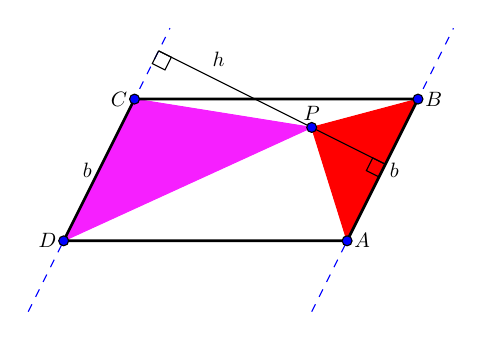
\begin{tikzpicture}
      \def\scale{4}
      \def\pr{\scale * 0.035}
      \def\pta{(\scale * 2, \scale * 0)}
      \def\ptb{(\scale * 2.5, \scale * 1)}
      \def\ptc{(\scale * 0.5, \scale * 1)}
      \def\ptd{(0, 0)}
      \def\ptp{(\scale * 1.75, \scale * 0.8)}
      \def\tscale{0.75}

      % Draw parallel extensions
      \draw[blue, dashed] (\scale * -0.25, \scale * -0.5) -- (\scale * 0.75, \scale * 1.5);
      \draw[blue, dashed, shift={(\scale * 2, 0)}] (\scale * -0.25, \scale * -0.5) -- (\scale * 0.75, \scale * 1.5);

      % Draw triangles
      \definecolor{colm}{rgb}{0.963,0.121,1}
      \draw[colm, fill=colm] \ptd -- \ptp -- \ptc -- cycle;
      \draw[red, fill=red] \pta -- \ptp -- \ptb -- cycle;

      % Perpendicular base line and right angle boxes
      \coordinate (A) at (\scale * 0.67, \scale * 1.34) {};
      \coordinate (B) at (\scale * 2.27, \scale * 0.54) {};
      \coordinate (Z) at (0, 0) {};
      \coordinate (SZ) at (\scale * 2, 0) {};
      \def\br{\scale * 0.1}
      \tkzMarkRightAngle[size=\br](Z,A,B);
      \tkzMarkRightAngle[size=\br](A,B,SZ);
      \draw (A) -- (B);

      % Draw parallelogram
      \draw[line width=1] \pta -- \ptb -- \ptc -- \ptd -- cycle;
      \draw[fill=blue] \pta circle (\pr);
      \node[anchor=west, scale=\tscale] at \pta {$A$};
      \draw[fill=blue] \ptb circle (\pr);
      \node[anchor=west, scale=\tscale] at \ptb {$B$};
      \draw[fill=blue] \ptc circle (\pr);
      \node[anchor=east, scale=\tscale] at \ptc {$C$};
      \draw[fill=blue] \ptd circle (\pr);
      \node[anchor=east, scale=\tscale] at \ptd {$D$};
      \draw[fill=blue] \ptp circle (\pr);
      \node[anchor=south, scale=\tscale] at \ptp {$P$};

      % Side labels
      \node[anchor=east, scale=\tscale] at (\scale * 0.25, \scale * 0.5) {$b$};
      \node[anchor=west, scale=\tscale] at (\scale * 2.25, \scale * 0.5) {$b$};
      \node[anchor=south west, scale=\tscale] at (\scale * 1, \scale * 1.175) {$h$};
    \end{tikzpicture}
  \end{center}
  Two sides of the parallelogram have length $b$ and the perpendicular line connecting these two sides has length $h$, and is of course the height of the parallelogram.
  Note that this line also intersects the common vertex of the two triangles, call this point $P$, and clearly has the same length $h$ regardless of where $P$ is placed.
  Clearly, also, the two segments of this line when split at $P$ also form the heights of the two triangles.
  Denote the area and height of the magenta triangle as $A_1$ and $h_1$, respectively.
  Similarly, denote the area and height of the red triangle $A_2$ and $h_2$, respectively.
  Hence, we have
  \gath{
    A_1 = \frac{1}{2} b h_1 \non
    A_2 = \frac{1}{2} b h_2 \non
    h = h_1 + h_2,
  }
  and the area of the parallelogram itself is $A = bh$.
  Therefore, the area of both triangles is
  \gath{
    A_1 + A_2 = \frac{1}{2} b h_1 + \frac{1}{2} b h_2 = \frac{1}{2} b (h_1 + h_2) = \frac{1}{2} b h = \frac{A}{2} = \frac{850}{2} = 425.
  }
  Note that this result is independent of the placement of $P$, and thus this is the smallest that this area $A_1 + A_2$ can be, and the largest for that matter since it is just constant.
}

\aproblem{21}{231}{\advent@xxii@xxi}{
  Clearly, this is simply the number of combinations of entrants when choosing two of them.
  So, if there are $n$ entrants, the number of matches is
  \gath{
    N(n) = \binom{n}{2} = \frac{n!}{2!(n-2)!} = \frac{n(n-1)}{2},
  }
  which are, interestingly, the triangular numbers such that
  \gath{
    N(n) = \frac{n(n-1)}{2} = \sum_{i=1}^{n-1} i.
  }
  Thus, our answer is simply $N(22) = 22 \cdot 21 / 2 = 231$.
}

\aproblem{22}{323}{\advent@xxii@xxii}{
  It is easy to simply continue this sequence manually:
  \gath{
    35 \non
    53 + 6 = 59 \non
    95 + 6 = 101 \non
    101 + 6 = 107 \non
    701 + 6 = 707 \non
    707 + 6 = 713 \non
    317 + 6 = 323.
  }
  Hence, evidently our answer is simply $323$.

  The computation of this sequence was verified with Python.
}

\aproblem{23}{125}{\advent@xxii@xxiii}{
  Clearly $1000$ does not qualify so that we need only consider $3$-digit numbers.
  Now, the set of invalid digits is $I = \braces{0, 1, 2, 3, 4}$ so that clearly the set of valid digits is $V = \braces{5, 6, 7, 8, 9}$, of which there are $5$.
  Since each valid number has exactly $3$ digits, clearly then there are $5 \cdot 5 \cdot 5 = 5^3 = 125$ of these since each digit can be any of the $5$ elements of $V$.

  This result was verified with a brute force Python program.
}

\aproblem{24}{128}{\advent@xxii@xxiv}{
  In general, the Binomial Theorem states that
  \gath{
    (x + y)^n = \sum_{k=0}^n \binom{n}{k} x^{n-k} y^k,
  }
  where of course
  \gath{
    \binom{n}{k} = \frac{n!}{k!(n - k)!}
  }
  is the binomial coefficient.
  In our case we have
  \gath{
    (3x - 1)^7 = \sum_{k=0}^7 \binom{7}{k} (3x)^{7-k} (-1)^k
  }
  so that clearly the sum of the coefficients is
  \gath{
    S = \sum_{k=0}^7 \binom{7}{k} 3^{7-k} (-1)^k .
  }
  While it would not be too hateful to expand this sum out by hand, we avoid this tedium and simply calculate the result using Python: $S = 128$.
}

\end{document}
